
%%%%%%%%%%%%%%%%%%%%%%%%%%%%%%%%%%%%%%%%%%%%%%%%%%%%%%%%%%%%%%%%%%%%%%%%
%Para las ecuaciones siempre es Ec.(n).
%Para las figuras siempre es Fig.n, incluso en el caption de la figura. Tambien las Tablas
%Para las referencias es [n]
%%%%%%%%%%%%%%%%%%%%%%%%%%%%%%%%%%%%%%%%%%%%%%%%%%%%%%%%%%%%%%%%%%%%%%%%

\documentclass[
reprint,
%notitlepage,
%superscriptaddress,
%groupedaddress,
%unsortedaddress,
%runinaddress,
%frontmatterverbose, 
%preprint,
%showpacs,preprintnumbers,
%nofootinbib,
%nobibnotes,
%bibnotes,
%11 pt,
amsmath,
amssymb,
aps,
pra,
%prb,
%rmp,
%tightenlines %esto hizo el milagro de sacar los espacios en blancos estocásticos (?)
 %prstab,
%prstper,
%floatfix,\textbf{}
]{revtex4-1} %Instalar primero para usarlo. Paquete malo.

%\documentclass[onecolumn, aps, amsmath,amssymb ]{article}
\usepackage{lipsum}  
\usepackage{graphicx}% Include figure files
\usepackage{subfig}
\usepackage{braket}
\usepackage{comment} %comment large chunks of text
\usepackage{dcolumn}% Align table columns on decimal point
\usepackage{bm}% bold math
%\usepackage{hyperref}% add hypertext capabilities
\usepackage[mathlines]{lineno}% Enable numbering of text and display math
%\linenumbers\relax % Commence numbering lines
\usepackage{mathtools} %% Para el supraíndice

\usepackage[nice]{nicefrac}

%%%%%%%El Señor Español%%%%%%%%%%%%%%%%%%%%%%%%%%%
\usepackage[utf8]{inputenc} %acento
\usepackage[
spanish, %El lenguaje.
es-tabla, %La tabla y no cuadro.
activeacute, %El acento.
es-nodecimaldot %Punto y no coma con separador de números
]{babel}
\usepackage{microtype} %para hacerlo más bonito :33 como vos (?) 
%%%%%%%%%%%%%%%%%%%%%%%%%%%%%%%%%%%%%%%%%%%%%%%%%%%
%%%%%%%%% Para que las imágenes se queden dónde las quiero (?
\usepackage{float}
%%%%%%%%%%

%%%%%%%%Cambia a Fig de Figure%%%%%%%%%%
\makeatletter
\renewcommand{\fnum@figure}{Fig. \thefigure} 
\makeatother
%%%%%%%%%%%%%%%%%%%%%%%%%%%%%%%%%%%%%%%%
\raggedbottom

\usepackage{hyperref}
\begin{document}
%%%%%%%%%%%%%%%%%%%%%%%%%%%%%%%%%%Título%%%%%%%%%%%%%%%%%%%%%%%%%%%%%%%%%%%%%%
%%%%%%%%%%%%%%%%%%%%%%%%%%%%%%%%%%%%%%%%%%%%%%%%%%%%%%%%%%%%%%%%%%%%%%%%%%%%%%

\title{Práctica 2: Dinámica de sistemas acoplados }
\author{Evelyn~G.~Coronel}

\affiliation{
Redes~Neuronales - Instituto~Balseiro\\}

\date[]{\lowercase{\today}} %%lw para lw, [] sin date

\begin{abstract}
Soluciones a los ejercicios de la práctica 2 de la materia de Redes Neuronales. En esta práctica se describe  la interacción entre neuronas como sistemas dinámicos acoplados.
\end{abstract} 
\maketitle
%%%%%%%%%%%%%%%%%%%%%%%%%%%%%%%%%%%%%%%%%%%%%%%%%%%%%%%%%%%%%%%%%%%%%%%%%%%%%%%%%%%

\section*{Ejercicio 1}

Las dos poblaciones de neuronas  están descritas por las siguientes ecuaciones:
\begin{align}
    \tau \nicefrac{df_e}{dt} &= -f_e + g_{ee} f_e\Theta(f_e) - g_{ei}f_i\Theta(f_i) + I_e\\
    \tau \nicefrac{df_i}{dt} &= -f_i + g_{ie} f_e\Theta(f_e) - g_{ii}f_i\Theta(f_i) + I_i
\end{align}
donde $f_i$ y $f_e$ son las tasas de disparo, $g_{ee}$ y $g_{ii}$ son las conductancias asociadas a la auto-interacción de la neuronas y los términos $g_{ie}$ y $g_{ei}$ son las conductancias de la interacción entre las neuronas.

Sabemos que la solución es estable cuando las derivadas se anulan
\begin{align}
    0= -f_e + g_{ee} f_e\Theta(f_e) - g_{ei}f_i\Theta(f_i) + I_e\\
    0= -f_i + g_{ie} f_e\Theta(f_e) - g_{ii}f_i\Theta(f_i) + I_i
\end{align}

Considerando que las tasas de disparo $f_e$ y $f_i$ son positivas y las conductancias  son mayores o iguales a 0,  las condiciones de estabilidad quedan como
\begin{align}
     (1 -g_{ee}) f_e &= -g_{ei}f_i + I_e \label{fe}\\
    (1 + g_{ii}) f_i &=  g_{ie} f_e  + I_i
\end{align}

Por lo que finalmente llegamos a un sistema de ecuaciones lineales para las tasas. Resolviendo este sistema, las tasas son iguales a 
\begin{align}
     f_i = (g_{ie}I_e + I_iA)(g_{ei}g_{ie}+ AB)^{-1}\\
     f_i = (g_{ei}I_i + I_eB)(g_{ei}g_{ie}+ AB)^{-1} 
\end{align}
donde $A= 1 - g_{ee}$ y $B=1+g_{ii}$. Como buscamos que las tasas sean positivas, los parámetro deben cumplir las siguiente relaciones: 

\begin{align}
     \frac{g_{ie}I_e + I_i -g_{ee}I_i }{1+g_{ei}g_{ie} - g_{ii}g_{ee} -g_{ee}-g_{ii}} > 0\\
     \frac{g_{ei}I_i + I_e +g_{ii}I_e }{1+g_{ei}g_{ie} - g_{ii}g_{ee} -g_{ee}-g_{ii}} > 0 .
\end{align}


\section*{Ejercicio 2}

\subsection{Introducción}

Las neuronas del tipo Hogdkin-Huxley se basan en las ecuaciones presentadas en \cite{HH}. En este trabajo, se agrega un parámetro $s$ que corresponde a la función inhibitoria \cite{syn} usada para modelar la inhibición sináptica. Este parámetro es descrito mediante la siguiente ecuación diferencial,
\begin{align}
    \frac{ds}{dt}&= \frac{s_\infty(V) - s}{\tau}\\
    s_\infty(V)&= 0.5(1+tanh(\nicefrac{V}{5})),
\end{align}
donde $V$ es el potencial de  la neurona y $\tau$ es el tiempo característico asociado a la inhibición. En este trabajo se considera  $\tau = 3\,$ms.

Para estudiar la interacción entre dos neuronas N-1 y N-2 del tipo Hogdkin-Huxley, consideramos que están conectadas simétricamente, es decir, la corriente $I(t)$ para ambas tiene de la forma
$I(t) = I_0 + I_{syn}(t) $ con 
\begin{equation}
     I_{syn}(t)      = -g_{syn}s(t)(V-V_{syn}),
 \end{equation} 
donde la corriente $I_0$ es valor tal que las dos neuronas produzcan spikes periódicamente, $s(t)$ es el parámetro descrito anteriormente, $g_{syn}$ es la conductancia asociada con la entrada sináptica y $V_{syn}$ es el potencial sináptico.

\subsection{Simulaciones}

   \subsubsection{Caso \texorpdfstring{$V_{syn}= 0\,\text{mV}$}{}   con  \texorpdfstring{$I_0 = 15\,\mu A$}{}}

En esta sección se varía el parámetro $g_{syn}$ entre $0$ y 2 ${\text{mS}}/{\text{cm}^2}$ con un paso de $\Delta g_{syn}=0.02\,{\text{mS}}/{\text{cm}^2}$ para un total 100 iteraciones. En cada iteración se mantiene fijo un valor para $V_{syn}$. La simulación de la evolución temporal de las neuronas utiliza $\Delta t =  0.005\,$ms y realizan $50000$ iteraciones, para un total de 250\,ms. En cada iteración de los valores de $g_{syn}$, las condiciones iniciales de las neuronas son tales que las mismas no estén en fase. Estás condiciones están dadas en la Tabla~\ref{tab:ini}.
\begin{table}[H]
    \centering
    \begin{tabular}{c| c| c |c |c|c}
     & V [mV] & m    & h     & n     & s     \\ \hline
    N-1       & 80      & 0.1  & 0.7   & 0.1   & 0.0   \\ \hline
    N-2       & -80     & 0.1  & 0.3   & 0.3   & 0.0  \\
   \end{tabular}
    \caption{Condiciones iniciales las neuronas del tipo Hodgkin-Huxley.}  
    \label{tab:ini} 
    \end{table}
Los parámetros adimensionales m, h y n están asociados a los canales de activación e  inactivación de sodio y al canal de potasio respectivamente.

En la Fig.\,\ref{fig:des_fre} se observan las curvas de la frecuencia y del desfase $\Theta$ de las dos neuronas en función de la conductancia $g_{syn}$. Los valores de la frecuencia y la conductancia se encuentra a la izquierda y derecha de la figura respectivamente. Se observa la disminución de la frecuencia de las neuronas con el aumento del valor de $g_{syn}$, debido a que la corriente $I_{syn}$ disminuye en media la corriente  $I(t)$ dentro de la neurona, esto es consistente con la curva f-I de las neuronas del tipo Hodgkin-Huxley, donde la frecuencia disminuye con la corriente en la neurona. 
        \begin{figure}[H]
            \centering
            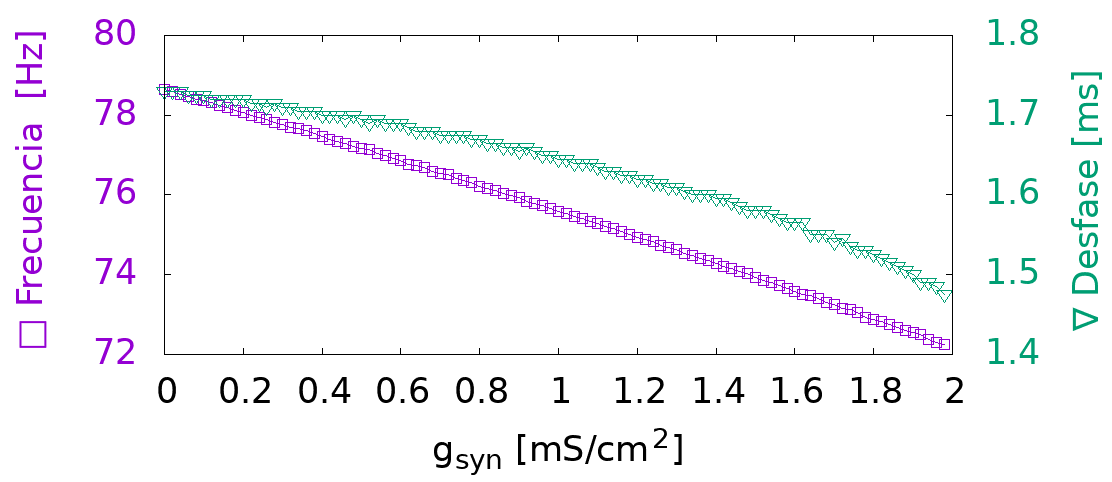
\includegraphics[width=0.5\textwidth]{current_15.png}
            \caption{Desfase y frecuencia de las neuronas en función de $g_{syn}$.}
            \label{fig:des_fre}
        \end{figure}  

Analizando la curva del desfase, se observa que este valor disminuye a media que aumenta el valor de $g_{syn}$. Por lo que aumentando este parámetro se obtiene $\Theta=0$\,s. 

\subsubsection{Caso \texorpdfstring{$V_{syn}= 80\,\text{mV}$}{}   con  \texorpdfstring{$I_0 = 15\,\mu A$}{}}



En esta sección se varía el parámetro $g_{syn}$ de la misma manera que la sección anterior. En la simulación de la evolución temporal se utiliza una variación de tiempo de $\Delta t =  0.01\,$ms y realizan $100000$ iteraciones, para un total de 1000\,ms. Para cada iteración de $g_{syn}$, las condiciones iniciales de las neuronas son tales que las mismas estén ligeramente desfasadas. Estás condiciones iniciales están dadas en la Tabla~\ref{tab:ini_in}.

\begin{table}[H]
    \centering
    \begin{tabular}{c| c| c |c |c|c}
    & V [mV] & m    & h     & n     & s     \\ \hline
    N-1       & 8      & 0.1  & 0.4   & 0.3   & 0.01   \\ \hline
    N-2       & -8     & 0.1  & 0.4   & 0.1   & 0.01  \\
   \end{tabular}
    \caption{Condiciones iniciales las neuronas del tipo Hodgkin-Huxley.}  
    \label{tab:ini_in} 
    \end{table}
%\begin{table}[H]
%    \centering
%    \begin{tabular}{c| c| c}
%    {\bf Variable }& {\bf Neurona 1} & { \bf Neurona 2} \\ \hline
%        V [mV]     & 8.0            & -8.0               \\  \hline
%        m          & 0.1             & 0.1              \\  \hline
%        h          & 0.4             & 0.4               \\  \hline
%        n          & 0.3             & 0.1               \\  \hline
%        s          & 0.01             & 0.01               \\      
%    \end{tabular}
%    \caption{Condiciones iniciales las neuronas del tipo Hodgkin-Huxley.}  
%    \label{tab:ini_in} 
%    \end{table}
   En la Fig.\,\ref{fig:des_fre_in} se observa que para valores pequeños de la conductancia $g_{syn}$ las neuronas empiezan con $\Theta= 0.06\,$ms. A medida que $g_{syn}$ aumenta su valor también aumenta $\Theta$, a diferencia del caso $V_{syn}=0\,$mV. Dado que $-\nicefrac{T}{2}<\Theta < \nicefrac{T}{2}$, alrededor de $g_{syn}=1.2\,\text{mS}/\text{cm}^2$ se observa una discontinuidad asociada al cambio del signo de $\Theta$. Así como también para otros valores de $g_{syn}$. Análogo al caso $V_{syn}=0\,$mV, la frecuencia disminuye con el $g_{syn}$, pero en este caso se debe al potencial inhibitorio que ralentiza la frecuencia de spikes de tal manera que los mismos estén desfasados.

   \begin{figure}[H]
            \centering
            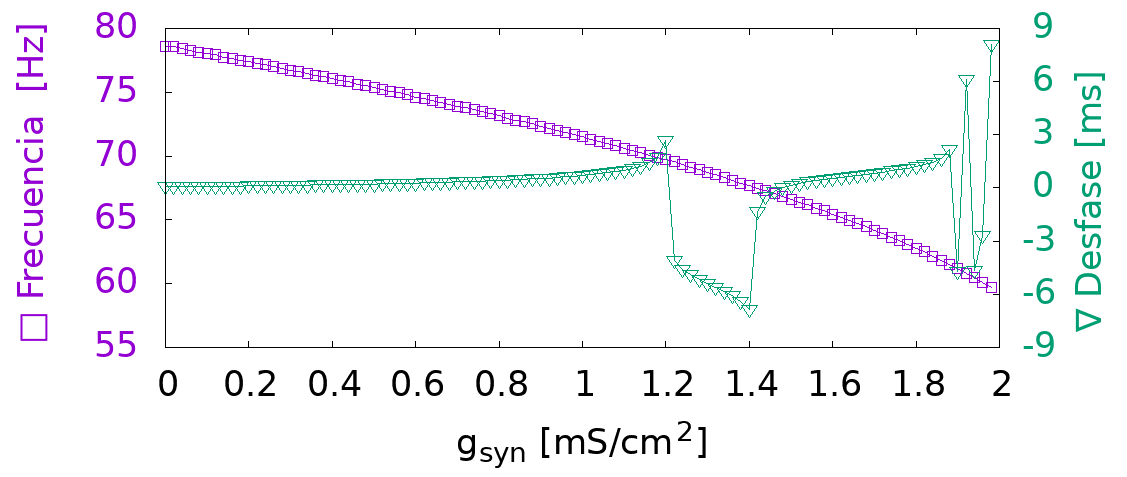
\includegraphics[width=0.5\textwidth]{current_15_in.png}
            \caption{Desfase y frecuencia de las neuronas en función de $g_{syn}$ para $V_{syn}=-80\,$mV.}
            \label{fig:des_fre_in}
        \end{figure}

    En las Figs.\, \ref{fig:gsyn0-1} y \ref{fig:gsyn1-2} se observan los spikes de ambas neuronas en función del tiempo para valores de $g_{syn}$ igual a $0.1\,\text{mS}/\text{cm}^2$ y $1.2\,\text{mS}/\text{cm}^2$ respectivamente. En la Fig. \ref{fig:gsyn0-1} se ve como los spikes están sincronizadas con un desfase despreciable. %, además que el valor de la corriente oscila sobre el valor de $I_0$ con una amplitud pequeña de $\approx 1.5\,\mu$A. 
    En cambio en la Fig.\,\ref{fig:gsyn1-2}, para $g_{syn}=1.2\,\text{mS}/\text{cm}^2$, los spikes están desfasados. 

     \begin{figure}[H]
        \centering
        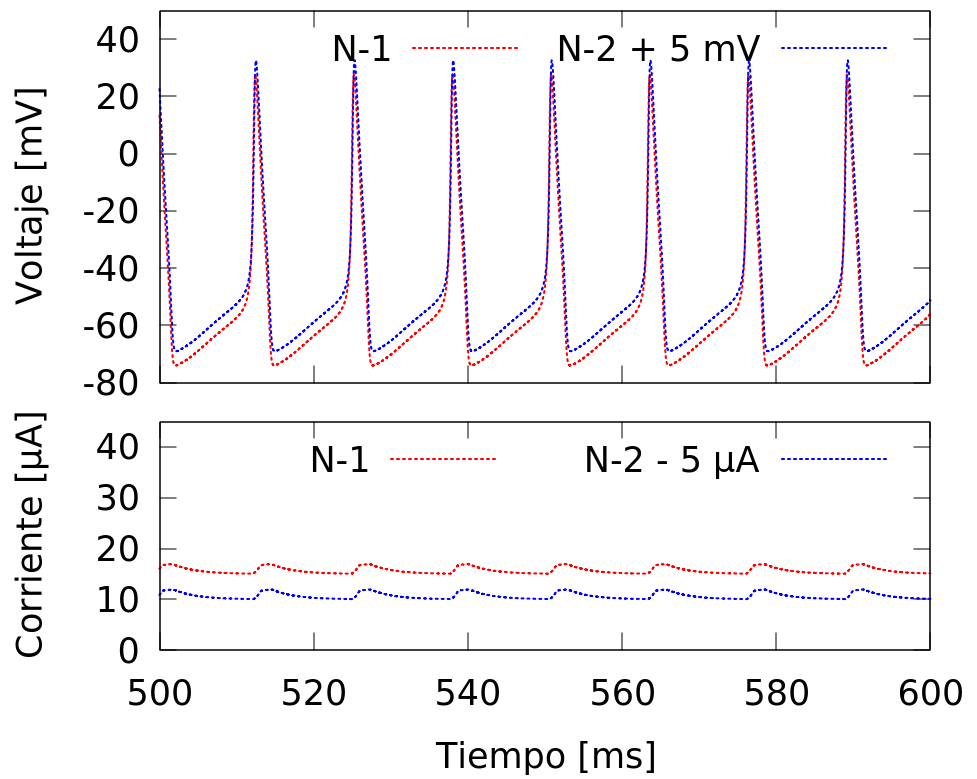
\includegraphics[width=0.415\textwidth]{current_15_in_gsyn_0-1.png}
        \caption{Curvas del voltaje y la corriente en función del tiempo para un valor de $g_{syn}=0.1\,\text{mS}/\text{cm}^2$}
        \label{fig:gsyn0-1}
    \end{figure}

        \begin{figure}[H]
        \centering
        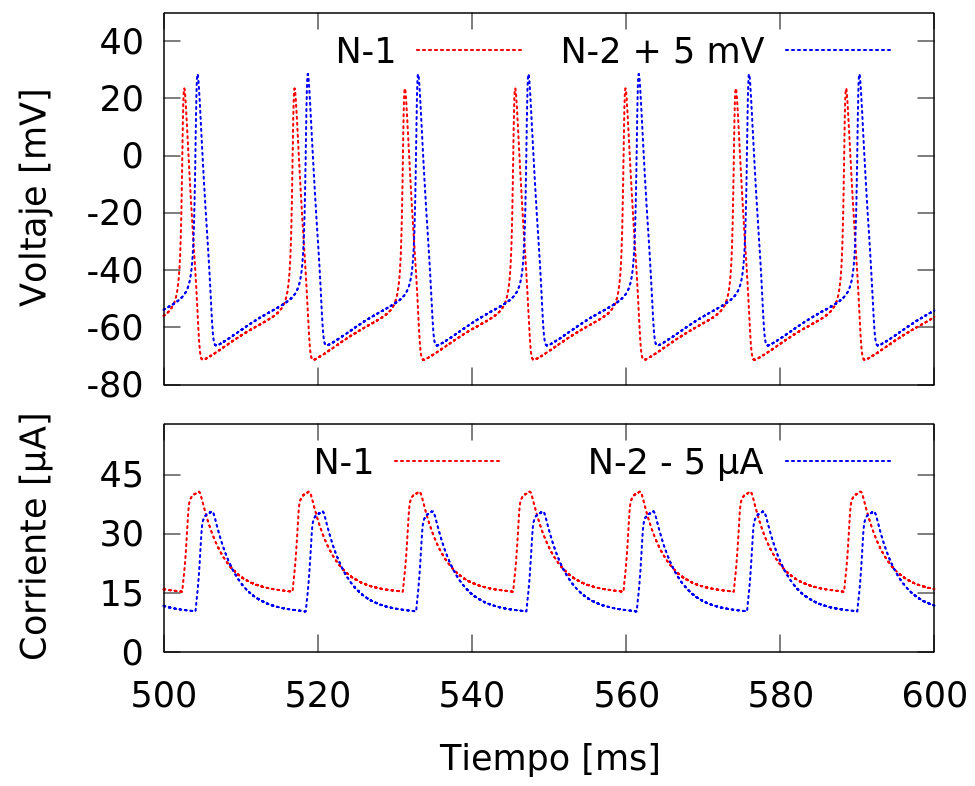
\includegraphics[width=0.415\textwidth]{current_15_in_gsyn_1-2.png}
        \caption{Curvas del voltaje y la corriente en función del tiempo para un valor de $g_{syn}=1.2\,\text{mS}/\text{cm}^2$}
        \label{fig:gsyn1-2}
    \end{figure}



\begin{thebibliography}{50}
%\onecolumn
\bibitem{HH} Izhikevich E. M. Capítulo 2. Sección 2.3: Hodgkin-Huxley Model en {\sl Dynamical Systems in Neuroscience: The Geometry of Excitability and Bursting} (2005).  The Neurosciences Institute.
\bibitem{syn} Börgers C, Krupa M, Gielen S. The response of a classical Hodgkin-Huxley neuron to an inhibitory input pulse. J Comput Neurosci. 2010;28(3):509–526. doi:10.1007/s10827-010-0233-8
\end{thebibliography}

\end{document}